\documentclass[10pt]{exam}
\usepackage[hon]{template-for-exam}
\usepackage{tikz,graphicx}
\usetikzlibrary{tikzlings}

\title{The Pig Lab}
\author{Rohrbach}
\date{\today}

\begin{document}
\maketitle

\vspace{-.7em}

\noindent
\emph{``I'll enjoy doing physics when pigs fly''}
\vspace{1em}

\noindent
Take out the pig and hang it from the ceiling.  Extend the wings, turn the pig on, allow it to run for a minute or so in order to watch its motion.

\begin{questions}
  
\question
  Turn the pig off.  Below, draw a free-body diagram of the pig in motion and label the forces in the correct directions (hint: they may not only go in the four cardinal directions.) 

  % \begin{tikzpicture}
  %   \tikzstyle{pigpath}=[dotted,thick]
  %   \tikzstyle{string}=[black!30]

  %   \begin{scope}
  %     \node at (0,4) {Side View};
  %     \coordinate (pig) at (2,0);
  %     \coordinate (vertex) at (0,3);
  %     \draw[string] (pig) -- (vertex);
  %     \fill (0,0) circle (.03);
  
  %     \begin{scope}
  %       \clip (-3,0) rectangle (1,.4);
  %       \draw[pigpath] (0,0) ellipse (2 and .4);
  %     \end{scope}
  
  
  %     \begin{scope}[shift={(2,-.4)}]
  %       \clip (-.75,0) rectangle (.75,1);
  %       \pig[shift={(0,-1.3)}]
  %     \end{scope}
  
  %     \begin{scope}
  %       \clip (-3,0) rectangle (3,-.4);
  %       \draw[pigpath] (0,0) ellipse (2 and .4);
  %     \end{scope}
  %   \end{scope}

  %   \begin{scope}[shift={(8,0)}]
  %     \node at (0,4) {Top View};
  %     \coordinate (pig) at (2,1.5);
  %     \coordinate (vertex) at (0,1.5);
  %     \fill (vertex) circle (.03);
  %     \draw[pigpath] (vertex) circle (2);
  
  
  %     \begin{scope}[shift={(2,.9)}]
  %       \clip (-.75,0) rectangle (.75,1);
  %       \pig[back,rotate=180,shift={(0,-2.3)}]
  %     \end{scope}

  %     \draw[string] (pig) -- (vertex);

  %   \end{scope}

  % \end{tikzpicture}

  %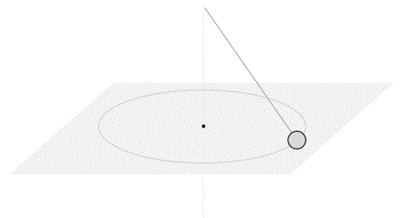
\includegraphics{flying-pig.png}

  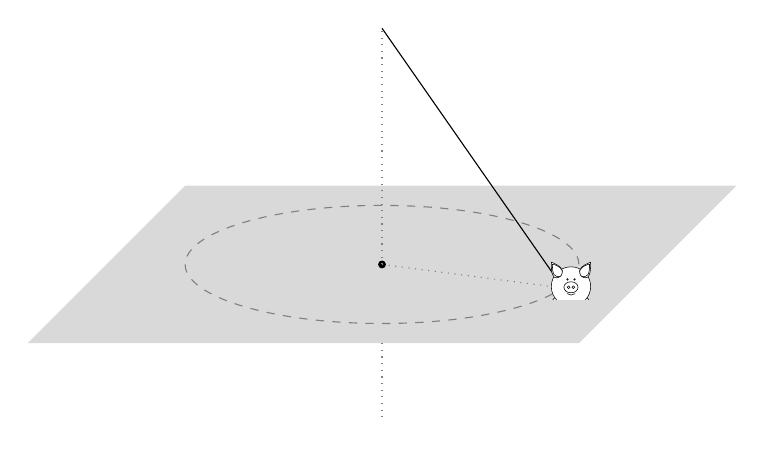
\begin{tikzpicture}
    \fill[gray!30] (0,0) -- 
      ++(7,0) -- 
      ++(2,2) --
      ++(-7,0) --
      cycle;
    \fill (4.5,1) coordinate (center)
      circle (0.05);
    \draw[dashed,gray] (center) 
      ellipse (2.5 and .75);
    \draw[dotted,gray] (center) 
      -- ++(0,3) coordinate (vertex);
    \draw[dotted,gray] (center) ++ (0,-1) -- ++(0,-1);
    \draw (6.8,.7) coordinate (pig) circle (0.1);
    \draw[dotted,gray] (center) -- (pig);
    
    \draw (vertex) -- (pig);

    %\draw (6.1,0) -- ++(2,2);

    \begin{scope}[shift={(pig)}]
      \begin{scope}[scale=0.5,shift={(.2,-.3)}]
          \clip (-.75,0) rectangle (.75,1);
          \pig[contour=black,shift={(0,-1.3)}]
      \end{scope}
    \end{scope}

  \end{tikzpicture}

  \vspace{5em}
  

\question
  Of the forces you drew in your diagram, which force is causing the centripetal force on the pig (\emph{hint:} think about the direction in which centripetal force acts)?
  \vs
  
\question
  What is the purpose of the $y$-component of the tension force?
  \vs

\question
  If the centripetal force is in towards the center, why does the pig seem to move out away from the string 
  \vs
  
\question
  What is the purpose of the wings?
  \vs 

\pagebreak

\uplevel{ Turn the pig back on and allow it to fly again so it is in a circle with a constant radius.}

\question
  Use a meter stick to estimate the radius of the pig's flight and record: 

  \vspace{1em}

  radius = \fillin[][6em] m

  \vspace{1em}

\question
  Time how long it takes the pig to make 10 complete revolutions and record: 

  \vspace{1em}
  
  total time of {\bf 10 revolutions} = \fillin[][6em] sec

  \vspace{1em}

\question
  Calculate the tangential speed of your flying pig.  
  \vs[2]

\question
  The pig's mass is approximately 0.4~kg.  Calculate its centripetal force.
  \vs


  


\end{questions}

\end{document}